% !TEX root = MAIN.tex

\section{Introduction}
\label{sec:introduction}
\addcontentsline{toc}{chapter}{Introduction}

%This document is the summary report of the ESA activity ITT-1-9873-ESA, which concerns the development of a framework for the automated assessment and the automated improvement of test suites for space software\footnote{In this report, we use the term space software to indicate software to be deployed on hardware that runs on-orbit.}.
 
From spacecrafts to ground stations, software has a prominent role in space systems; for this reason, the success of space missions depends on the quality of the system hardware as much on the dependability of its software. Mission failures due to insufficient software sanity checks~\cite{Schiaparelli} are unfortunate examples, pointing to the necessity for systematic and predictable quality assurance procedures in space software. 


Existing standards for the development of space software regulate software quality assurance and emphasize its importance. 
The most stringent regulations are the ones that concern flight software, i.e., embedded software installed on spacecrafts, our target in this activity.
In general, software testing plays a prominent role among  quality assurance activities for space software, and standards put a strong emphasis on the quality of test suites. For example, the European Cooperation for Space Standardization (ECSS) provides detailed guidelines for the definition and assessment of test suites~\cite{ecss80C,ecss40C}. 

Test suites assessment 
is typically based on code inspections performed by space authorities and
independent software validation and verification (ISVV) activities, which include the verification of test procedures and data (e.g., ensure that all the requirements have been tested and that representative input partitions have been covered~\cite{ISVV}). Though performed by specialized teams, such assessment is manual and thus error prone and time-consuming. \EMPH{Automated and effective methods to evaluate the quality of the test suites are thus necessary.}
 Also, \EMPH{methods to automatically generate test cases will speed-up the improvement of test suites}. 

Since one of the primary objectives of software testing is to identify the presence of software faults, an effective way to assess the quality of a test suite consists of artificially injecting faults in the software under test and verifying the extent to which the test suite can detect them. 
This approach is known as \emph{mutation analysis}~\cite{DeMillo78}. 
In mutation analysis, faults are automatically injected in the program through automated procedures referred to as mutation operators. Mutation operators enable the generation of faulty software versions that are referred to as \emph{mutants}.  
Mutation analysis helps evaluate the effectiveness of a test suite, \JMRCHANGE{for a specific software system,} based on its mutation score, which is the percentage of mutants leading to test failures.

Despite its potential, mutation analysis is not widely adopted by industry in general and space system development in particular. The main reasons include its limited scalability and the pertinence of the mutation score as an adequacy criterion~\cite{papadakis2016threats}. Indeed, for a large software system, the number of generated mutants might prevent the execution of the test suite against all the mutated versions. Also, the generated mutants might be either 
semantically equivalent to the original software~\cite{madeyski2013overcoming} or redundant with each other~\cite{Shin:TSE:DCriterion:2018}.
Equivalent and redundant mutants may bias the mutation score as an adequacy criterion. 

The mutation analysis literature has proposed several optimizations to address problems related to scalability and mutation score pertinence. 
For example, scalability problems are addressed by approaches that sample mutants~\cite{zhang2013operator}~\cite{gopinath2015hard}
or solutions that prioritize and select the test cases to be executed for each mutant~\cite{zhang2013faster}. Equivalent and redundant mutants can be detected by comparing the code coverage of the original program and its mutants~\cite{grun2009impact,schuler2010covering,schuler2013covering,schuler2009efficient}. 
However, these approaches 
have not been evaluated on industrial, embedded systems
and there are no feasibility studies concerning the integration of such optimizations and their resulting, combined benefits.
For example, we lack mutants sampling solutions that accurately estimate the mutation score in the presence of reduced test suites;
indeed, mutant sampling, which comes with a certain degree of inaccuracy, may lead to inaccurate results when applied to reduced test suites that do not have the same effectiveness of the original test suite.

In addition, existing mutation analysis approaches cannot identify problems related to the interoperability of integrated components (integration testing).
Space software, similar to software running in other types of CPSs, is often affected by problems cause by the lack of  \INDEX{interoperability of integrated components}~\cite{Givehchi:2017,Jirkovsk:2017}, mainly due to the wide variety and heterogeneity of the technologies and standards adopted.
It is thus of fundamental importance to ensure the effectiveness of test suites with respect to detecting interoperability issues, for example by making sure test cases trigger the exchange of all possible data items and report failures when erroneous data is being exchanged by software components. For example, the test suite for the control software of a satellite shall identify failures due to components working with different measurement systems~\cite{MarsClimateOrbiter}.
Unfortunately, well known, code-driven mutation operators (e.g., the sufficient set~\cite{delamaro2014designing,delamaro2014experimental}) simulate algorithmic faults by introducing small changes into the source code and are thus unlikely to simulate interoperability problems resulting in \UPDATED{exchanges of erroneous data}. 

Finally, traditional mutation analysis approaches  \emph{cannot inject faults into black-box components} whose implementation is not tested within the development environment (e.g., because it is simulated or executed on the target hardware).
For example, in a satellite system, such components include the control software of the Attitude Determination And Control System (ADCS), the GPS, and the Payload Data Handling Unit (PDHU). During testing with simulators in the loop, the results generated by such components (e.g., the GPS position) are produced by a simulator. During testing with hardware in the loop, these components are directly executed on the target hardware and cannot be mutated, either because they are off-the-shelf components 
or to avoid damages potentially introduced by the mutation.

Last, test generation approaches are in preliminary stages and cannot be applied in industrial space context. For example, SEMU, a state-of-the-art approach can generate test inputs only for batch programs that can be compiled with the LLVM infrastructure.

FAQAS had the objective to assess the feasibility of mutation analysis and testing for space software by identifying feasible solutions based on existing literature. FAQAS objectives were the following:
\begin{itemize}
\item To perform a comprehensive analysis and survey of mutation analysis/testing.
\item To prototype the mutation analysis/testing process to be applied on space software. 
\item To develop a toolset supporting mutation analysis and testing automation.
\item To empirically evaluate mutation analysis/testing by applying it to space software use cases. 
\item To evaluate how mutation analysis/testing can be integrated into a typical verification and validation life cycle of space software and to define a mutation analysis/testing methodology. 
\end{itemize}


\subsection*{Overview of the contributions}

The FAQAS activity addresses the problems above. It is a joint work between the SnT Centre of the University of Luxembourg\footnote{https://wwwen.uni.lu/snt}, Gomspace Luxembourg\footnote{https://gomspace.com/} (GSL) and OHB Luxspace\footnote{https://luxspace.lu/} (LXS).
FAQAS led to the development of a toolset that addresses the challenges above. It includes four tools:
\EMPH{MASS} (Mutation Analysis for Space Software), 
\EMPH{DAMAt} (DAta-driven Mutation Analysis with Tables), 
\EMPH{SEMuS} (Symbolic Execution-based MUtant analysis for Space software),
and \EMPH{DAMTE} (DAta-driven Mutation TEsting).



% of code-driven mutation analysis in the space context. The evaluation has shown that the most effective solutions to improve scalability and mutation score accuracy are mutants sampling and equivalence metrics based on compiler optimizations, respectively. To guarantee a scalable mutation testing process and the accurate computation of the mutation score, mutants sampling should be based on sequential analysis relying on fixed-width sequential confidence interval, a research discovery done within FAQAS.
%
%•	An empirical evaluation demonstrating the feasibility of data-driven mutation analysis with space software.
%•	The definition of an approach for code-driven mutation testing that relies on symbolic execution to identify test inputs that enable killing mutants not killed by the test suite under analysis.
%•	Demonstrating the feasibility of automated test generation for mutation testing based on symbolic execution. More precisely, symbolic execution can be successfully used to select test inputs that kill live mutants within unit test cases. However, unsurprisingly, it cannot be adopted when, to kill a mutant, it is necessary to rely on external components (e.g., networks or simulators), in such cases, which are common for integration and system test suites, symbolic execution alone is insufficient to generate test cases (e.g., because it cannot translate the simulator logic into an SMT formula to derive test cases from).
%\item The definition of guidelines for the adoption of mutation analysis and testing strategies within ECSS activities. The proposed guidelines support both quality assurance activities described in ECSS standards and Independent Software Verification and Validation (ISVV) practices.
%\end{itemize}

\begin{figure*}[tb]
\begin{center}
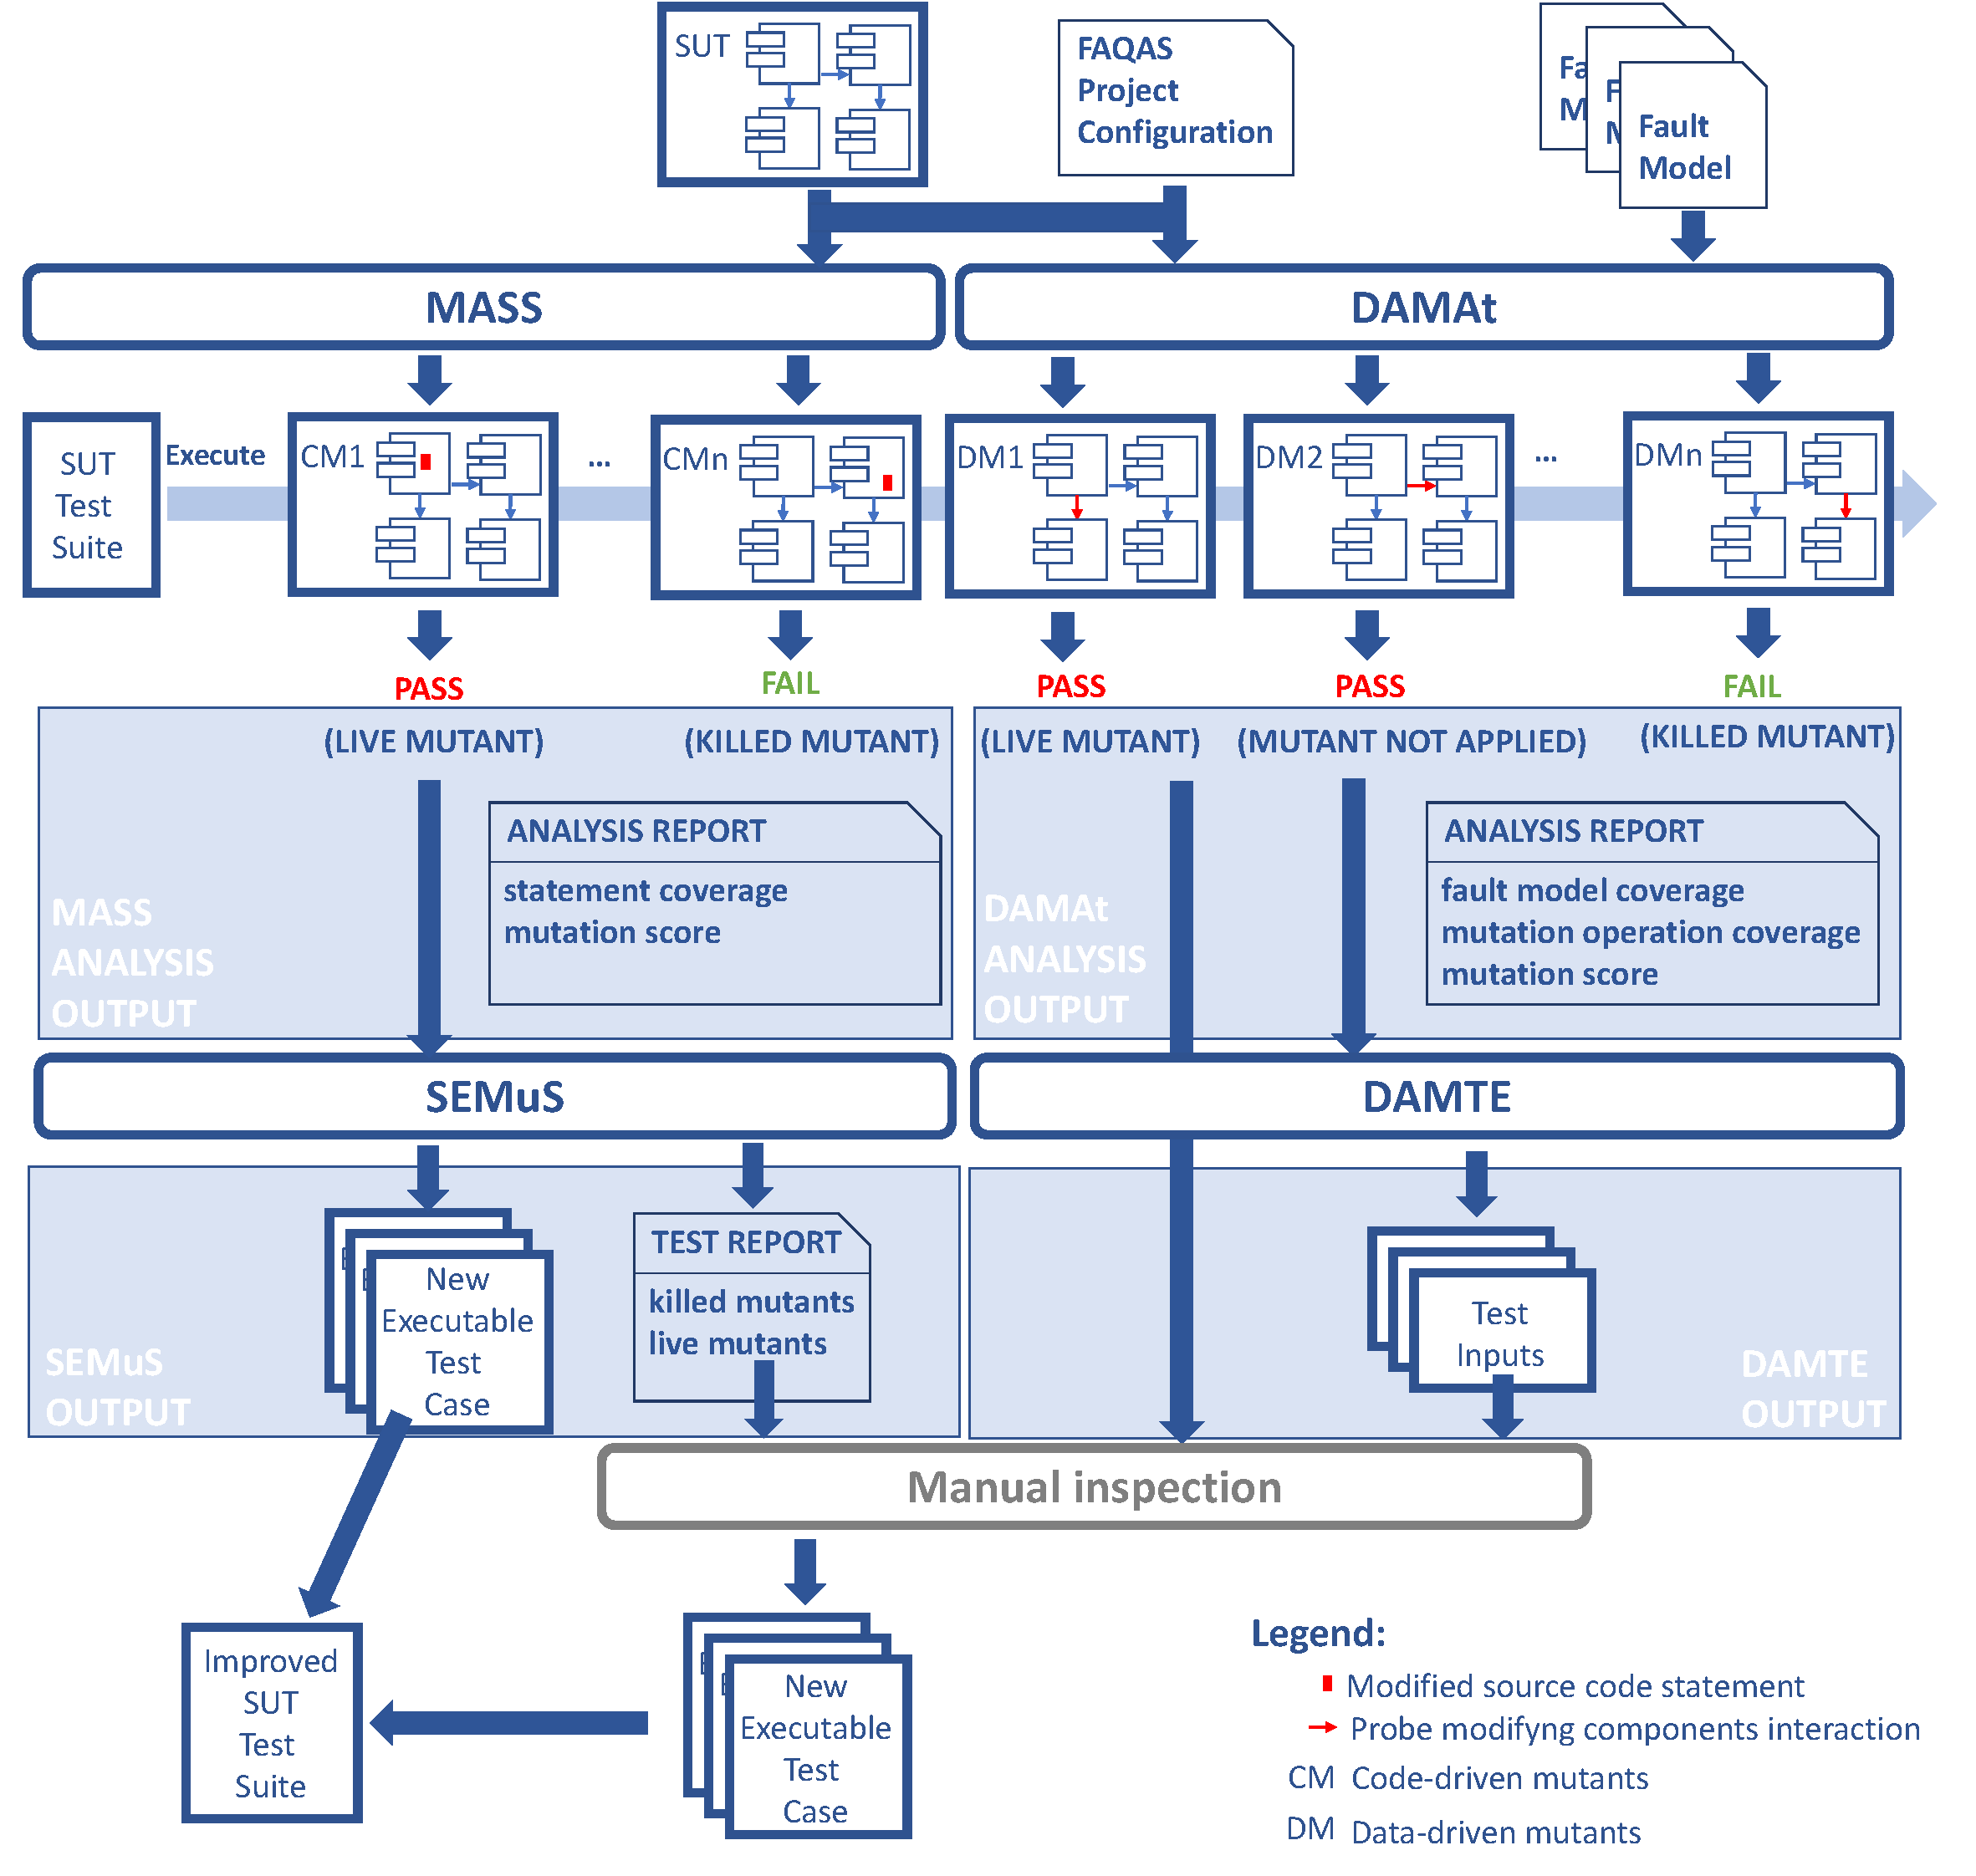
\includegraphics[width=\textwidth]{images/FAQAS-overview.pdf}
\caption{Overview of the FAQAS toolset}
\label{fig:FAQAS:toolset}
\end{center}
\end{figure*}

Figure~\ref{fig:FAQAS:toolset} provides an overview of the input and outputs of the FAQAS toolset. It relies on the idea of generating multiple modified versions of the software system under test (SUT), some are derived by modifying the implementation of the software (code-driven mutants) other by integrating a mutation API that alters the messages exchanged by the software components of the SUT (data-driven mutants). 
The SUT test suite shall be executed with all the mutants, if it is effective then it shall fail with each of them. The mutants for which a failure is not observed are said to be \EMPH{live} and indicate a pitfall in the test suite.
All the FAQAS tools take as input the software under test (SUT), its test suite, and a set of configuration files. 

\EMPH{MASS} generates code-driven mutants. It integrates a pipeline of solutions that make mutation analysis feasible wit large SUT. The three main contributions of MASS are (1) the automated identification of trivially equivalent mutants using an ensemble of compiler optimization options, (2) the computation of the mutation score based on mutant sampling with fixed size confidence interval approach (FSCI), (3) the automated identification of equivalent mutants based on coverage. 
MASS reports the set of live mutants, the set of killed mutants (i.e., mutants that are discovered by the test suite), and information useful to draft a verification report, which includes the statement coverage of the SUT test suite and the mutation score (i.e., the percentage of mutants discovered by the test suite).

\EMPH{DAMAt} generates mutants for data-driven mutation analysis. Data-driven mutation analysis is a research contribution of FAQAS. Instead of mutating the implementation of the SUT, it consists of altering the data exchanged by software components. 
DAMAt relies on fault models that specify how to mutate the data exchanged by software components through data-driven mutation operators. DAMAt can automatically alter data that is stored in data buffers (e.g., before serialization on the communication channel).
DAMAt enables the simulation of faults that affect simulated components (e.g., sensors), which is not feasible with traditional, code-driven mutation analysis. 
DAMAt generates as output a set of killed mutants (i.e., mutants that, during testing, successfully alter the data, and lead to test case failures), a set of live mutants (i.e., mutants that, during testing, successfully alter the data, but do not lead to test case failures), and a set of mutants not applied (i.e., mutants that, during testing, could not alter any data because the data they target is never exercised by the SUT); also, it provides information useful to draft a verification report, which includes the fault model coverage (i.e., percentage of fault models with at least one mutant applied), the mutation operation coverage (i.e., percentage of mutants applied), and the mutation score.

\EMPH{SEMuS} automatically generates executable unit test cases based on code-driven mutation analysis results. The generated unit test cases detect mutants not detected by the original test suite. The generated test cases include test oracles that shall be manually validated by engineers, which enables detecting faults. The generated test cases can be integrated into regression test suites.

SEMuS takes as input the list of live mutants detected by MASS. It generates a set of additional test cases that can be integrated into the SUT test suite. Also, it reports the list of killed mutants and the list of mutants that remain live (i.e., for which SEMuS did not generate a test case that kill them). Live mutants shall be manually inspected by engineers to either determine if they are equivalent or to manually derive a test case capable of killing them.

\EMPH{DAMTE} is a manual procedure supported by an automated symbolic execution toolset; it automatically identifies the test inputs that make software components exchange the data targeted by data-driven mutation operators. The derived test inputs can then be manually integrated into the SUT test suite.
 
The activity also included an extensive empirical evaluation demonstrating the feasibility, effectiveness, and scalability of the proposed toolsets in the space context, as described in the following sections.

Sections~\ref{ch:mass:approach} to~\ref{sec:data:test_suite_augmentation} provide an overview of the FAQAS tools: MASS, SEMuS, DAMAt, and DAMTE.
Section~\ref{chapter:caseStudies} introduces the case study subjects considered for empirical evaluation.
Section~\ref{sec:summary:results} provides an overview of the empirical results obtained.
Section~\ref{sec:conclusion} concludes this report.

